\section{Logik}
Neben den Klassen, in denen die Fenster beschrieben werden, existieren auch Klassen in denen die Logik beschrieben steht. Diese werden in diesem Unterkapitel behandelt.

\subsubsection{Project-Klasse}
Die \textit{Project}-Klasse stellt ein FM3D-Projekt dar. Es besitzt Methoden, um Projekte aus \ac{XML}-Dateien zu laden, in \ac{XML}-Dateien zu speichern und den Projektnamen zu setzen. Zudem besitzt es eine Instanz zu dem gerade aktiven Projekt und den Projektnamen und das Verzeichnis in Form des Datentyps \textit{String}. Auf die Unterverzeichnisse kann man durch ein Objekt der \textit{RootDirectory}-Klasse\cref{rootdirectory} zugreifen.

\subsubsection{RootDirectory-Klasse}
\label{rootdirectory}
Diese Klasse erbt von der Klasse \textit{Directory} (Siehe \cref{directory}) und stellt das sogenannte Wurzelverzeichnis dar. Sie besitzt ein Boolean, mit dem dargestellt wird, ob das Verzeichnis im FileBrowser (Siehe \cref{filebrowser}) angezeigt werden kann.

\subsubsection{Directory-Klasse}
\label{directory}
Die \textit{Diretory}-Klasse besitzt drei \textit{ObservableCollections} in Form von Objekten der Klassen \textit{FileObject}, \textit{File} und \textit{Directory}. Dadurch dass die Directory-Klasse \textit{ObservableCollections} des eigenen Types hat, kann eine simple Baumstruktur von Ordner gebildet werden. Sie erbt von der \textit{FileObject}-Klasse. \cref{fileobject}

\subsubsection{File-Klasse}
Diese Klasse erbt auch von der \textit{FileObject}-Klasse. Sie wird in der \textit{Directory}-Klasse verwendet um die Projektdateien zu beschreiben.

\subsubsection{FileObject-Klasse}
\label{fileobject}
Diese Klasse beschreibt die Grundstruktur eines Objektes, welches in einer Ordnerstruktur bzw. in einem FM3D-Projekt dargestellt wird. Der Dateiname und Dateipfad werden durch den Datentyp String beschrieben.

\subsubsection{Filebrowser View-Logic}
\label{fbview}
Die Klasse \textit{Logic}, welche im Namespace "`\textit{FM3D\_Designer.src.ToolWindows.FileBrowser}"' steht, erbt von dem Interface \textit{INotifyPropertyChanged}. \textit{INotifyPropertyChanged} ist ein Interface, womit Events gefeuert werden können, wenn sich eine bestimmte Eigenschaft ändert, sodass andere Klassen wie zb. ein Fenster darauf reagieren können.
Dies benutzt man hier, um \todo{!!!}
Die Klasse enthält eine Enumeration, welche die Anzeigeeinstellung des File-Browser beschreibt. 
Eine in der Klasse \textit{Logic} stehende \textit{ObservableCollection} enthält alle Wurzelverzeichnisse, welche mit der Klasse \textit{Item} beschrieben werden. In einem Objekt der Klasse \textit{Item} namens \textit{\_CurrentDirectory} und der Eigenschaft \textit{CurrentDirectory}, welche das \textit{Item}-Objekt von \textit{\_CurrentDirectory} zurück gibt, wird das aktuelle . Ein Interface vom Typ \textit{IList} gibt den Inhalt der aktuell ausgewählten \textit{Directory} im File-Browser (Siehe \cref{filebrowser}) zurück. Zudem besitzt diese Klasse verschiedene Methoden zur Interaktion mit dem File-Browser.

\subsubsection{Item}
\label{item}
Objekte der Klasse \textit{Item} sind dafür , im \textit{File-Browser} angezeigt zu werden. Die Klasse erbt von dem Interface \textit{INotifyPropertyChanged}, welches schon in \cref{fbview} erläutert wurde. Ein \textit{Item} besitzt eine Enumeration namens \textit{ItemState}, welche angibt, ob das Item im Projekt eingebunden, nicht eingebunden wurde oder nicht in der Ordnerstruktur gefunden wird. Es besitzt zudem ein Objekt der Klasse ItemType, um den Typ der Datei anzugeben, und ein Objekt der Klasse Logic. So kann auch hier, ähnlich wie bei der Klasse \textit{Directory}, eine Baumstruktur gebildet werden.
%%  Dictionary<ItemType, List<Item>>
Ein rekursives Objekt der Klasse Item gibt das \textit{Parent}-Item an. Dies ist das \textit{Item}, welches das übergeordnete Verzeichnis angibt.
Ein Item besitzt zudem ein \textit{ContextMenu}, welches bei einem Rechtsklick auf das Item geöffnet wird. Des weiteren wurden Methoden Implementiert, welche verschiedene Dialoge und Fenster öffnen. Man kann durch sie den \textit{Text-Editor}, den \textit{Entity-Editor} und den \textit{AddNewResource}-Dialog öffnen, welche sofort mit diesem \textit{Item} interagieren.
Die Methode \textit{CreateFile} kann mit Angabe eines Dateinamen, einem \textit{ItemType} und dem \textit{Item}, das gerade angeklickt ist, eine neue Datei erstellen. Dies geschieht im Programm über das \textit{ContextMenu} durch den \textit{AddResource}-Dialog.

\subsubsection{ItemType}
Diese Klasse gibt den Typ eines Item an. Sie besitzt einen Container in Form eines \textit{Dictionary}. Als Schlüsselwert/Key wird ein String verwendet. Der Wert/Die Value ist ein Rekursives Objekt der selbigen Klasse \textit{ItemType}.
In ItemType stehen statische einzelne rekursive Objekte der selbigen Klasse für jeden Dateien-Typ den es in dem FM3D-Projekt existiert.
Jeder Typ besitzt Pfade zu den Icons, welche im File-Browser angezeigt werden.  Es existieren insgesamt acht verschiedene:
\begin{itemize}
	\item Directory
	\item UnknownFile
	\item EntityFile
	\item MaterialFile
	\item SkeletonFile
	\item MeshFile
	\item TextureFile
	\item ModelFile
\end{itemize}


\subsubsection{Entity-Klassen}
\label{entityklassen}
Sowohl im Designer als auch in der Extension gibt es jeweils die selben drei Klassen, welche für die Entities zuständig sind: \textit{Entity}, \textit{Component} und \textit{Property}.
Die \textit{Entity} Klasse beschreibt das Entity, so wie sie später im Code erstellt werden sollen. Ein Entity-Objekt besitzt einen Namen und drei Container des Typen \textit{List}. Die erste Liste besitzt Objekte der Klasse \textit{Component}, die zweite und dritte Liste sind Objekte der Klasse \textit{Property} und sind jeweils für die automatisch generierten und für die benutzerdefinierten Properties.
Jeder dieser Klassen besitzt zudem eine überladene \textit{ToString()} Methode, welche dafür sorgt, dass alle Daten in ein String geschrieben werden, um sie dann später per Pipe zu verschicken.
Um die einheitliche Trennung der Daten durch verschiedene \textit{Chars} in diesem zu versendenden Stringdatensatz zu gewährleisten wurde die statische Klasse \textit{SC} implementiert, welche die Trennungszeichen beinhaltet.
Jeder dieser drei Klassen -die statische Klasse \textit{SC} zählt nicht dazu, da sie nur eine Sammlung von Zeichen zur Trennung sind- enthalten noch einen Konstruktor, welcher einen umgewandelten Datensatz vom Typ String wieder in eines dieser Objekte umwandelt. 
So können, nachdem ein Entity in Form eines Datensatzes vom Typ String per Pipe an die VisualStudio-Extension geschickt wurde, die Daten dort weiterverwendet werden. 
Die Klassen werden in \cref{entityklassendiag} dargestellt.
\begin{figure}
	\begin{center}
		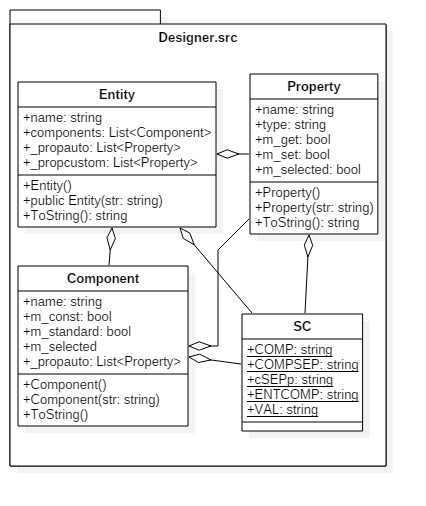
\includegraphics[width=0.4\textwidth]{03unserprogramm/Designer/EntityKlassen.png}
		\caption{Entity-Klassen im Designer}\label{entityklassendiag}
	\end{center}
\end{figure}

\subsubsection{Creator}
Um ein Item zu erstellen muss die Klasse Creator verwendet 
\todo[inline]{!!!}
\subsubsection{FM3DPropertyFile-Klasse}
Diese Klasse ist dafür zuständig, Daten aus der Datei \textit{fm3d.xml} zu lesen. Diese Datei beinhaltet Daten für die Kommunikation mit der Extension per Pipe. Sowohl im Designer als auch in der Extension sind zwei von der Grundstruktur sich ähnelnde Klassen der \textit{FM3DPropertyFile}-Klasse.

\subsubsection{PipeSystem} 
\label{pipe}
Grob betrachtet ist die Pipe eine Klasse, welche die Kommunikation zwischen zwei Programmen ermöglicht. In unserem Fall kommunizieren der FM3D-Designer und die dazugehörige VisualStudio-Extension\ref{extension}. Das ganze läuft relativ ähnlich wie bei simpler Netzwerkkommunikation ab. 
Sowohl im Designer als auch in der Extension sind von der Grundstruktur sich ähnelnde Klassen des PipeSystems.

\subsubsection{FM3D-Extension}
\label{extension}
Die FM3D-Extension ist eine von uns entwickelte Erweiterung für VisualStudio. Sie ist dafür zuständig gesendete Entities\ref{entityklassen} in C++ Code umzuwandeln. In \cref{vsextensiondia} wird der Aufbau der Extension dargestellt.
\begin{figure}
	\begin{center}
		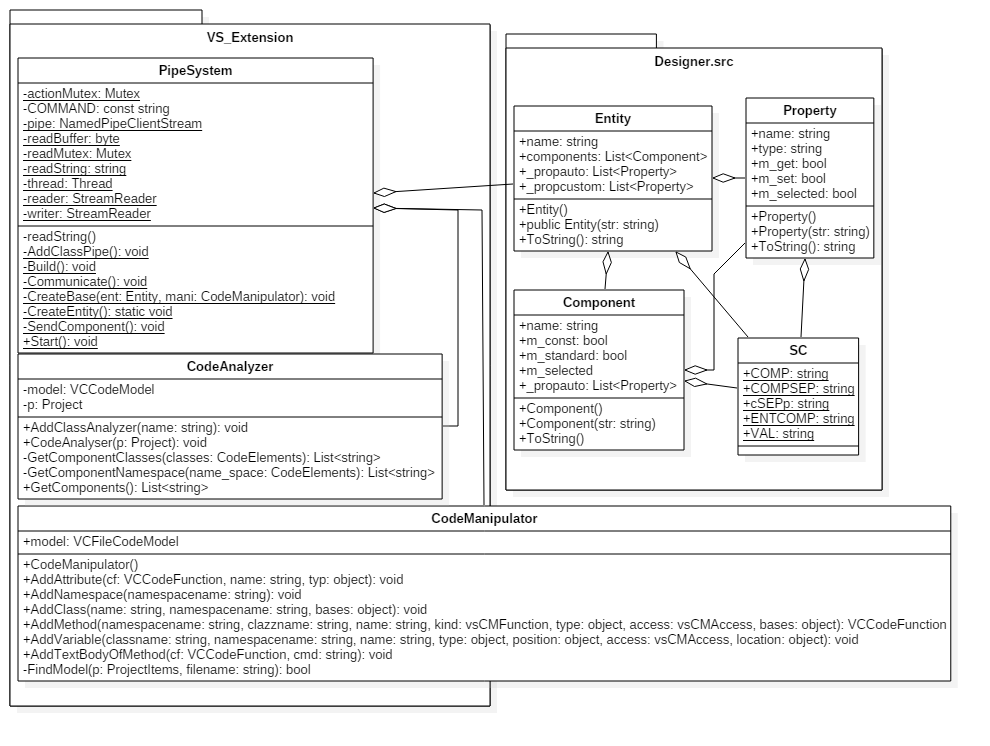
\includegraphics[width=\textwidth]{03unserprogramm/Designer/VSExtension.png}
		\caption{VisualStudio-Extension}\label{vsextensiondia}
	\end{center}
\end{figure}